\documentclass[12pt,letterpaper]{article}
\usepackage[utf8]{inputenc}
% AMS packages
\usepackage{amsmath}
\usepackage{amsfonts}
\usepackage{amssymb}
% no indent at new paragraph
\usepackage[parfill]{parskip}
% to include figures 	
\usepackage{graphicx}
% for consistent SI units
\usepackage{siunitx}
\sisetup{%
  output-decimal-marker={.},
  load-configurations=abbreviations,
  %group-separator={,},
  sticky-per=true,
  %per-mode=fraction
  per-mode=symbol
}
% to hyperlink figure and equation numbers in a pdf correctly
\usepackage[colorlinks=false, pdfborder={0 0 0}]{hyperref}
\usepackage[all]{hypcap}
% to make math larger and smaller
\usepackage{relsize}
\begin{document}

\title{Simulating Laminar Flow over a Flat Plate with an Isothermal Wall in SU2}
\author{Kedar R. Naik \\
 Stanford University \\
 \texttt{knaik@stanford.edu}}
\date{\today}
\maketitle

\begin{abstract}
Several simulations of flat-plate flow were performed using SU2 at NASA Glenn from June to July of 2014. Here, one specific case has been investigated again, namely: laminar flow over a flat plate with an isothermal wall boundary condition. Two different wall temperatures have been studied --- one where the temperature difference between the freestream and the surface is relatively small, $\SI{3}{\kelvin}$, and  where is it relatively large, $\SI{50}{\kelvin}$. In both cases, a low freestream Mach number has been chosen in an attempt to minimize the effects of compressibility. Various quantities of interest from these two simulation have been plotted. Where appropriate, the computational results have been compared with analytical solutions. The purpose of this report is to assist work on thermal boundary layers that is currently ongoing at NASA Glenn.
\end{abstract}

\section*{Preliminaries}
The physical flow parameters of these simulations, as well as the numerical methods used, are described below.

\subsection*{Flow Conditions}
This case simulates the laminar flow of air ($\gamma$ = 1.4) over a flat plate held at a constant temperature, $T_w$. Here, two separate wall temperatures have been considered, i.e.

\begin{align*}
&\mathrm{Case \, I}: & T_w = \SI{303}{\kelvin} \\
&\mathrm{Case \, II}: & T_w = \SI{350}{\kelvin}
\end{align*}

Other specific conditions of the flow are listed below.

\begin{align*}
&c_p = \SI{1005}{\joule\per\kilogram\kelvin} & \text{specific heat capacity} \\
&k = \SI{0.02618}{\watt\per\meter\kelvin} & \text{thermal conductivity} \\
&p_{t_{in}} = \SI{100000}{\pascal} & \text{inlet stagnation pressure} \\
&p_{out} = \SI{99303.1}{\pascal} & \text{outlet static pressure} \\
&Pr = 0.72 &\text{Prandtl number} \\
&T_{t_{in}} = \SI{300}{\kelvin} & \text{inlet stagnation temperature} \\
&T_\infty = \SI{300}{\kelvin} & \text{freestream temperature} \\
&U_\infty = \SI{34.7715}{\meter\per\second} & \text{freestream velocity}\\
&\mu = \SI{1.84492e-5}{\newton\second\per\meter\squared} & \text{dynamic viscosity} \\
&\rho_\infty = \SI{1.13753}{\kilogram\per\meter\cubed} & \text{freestream density}
\end{align*}

N.B. The static pressure at the outlet, $p_{out}$, was computed using the isentropic relation, viz.

\begin{equation*}
p_{out} = p_{t_{in}}\left[ 1+\dfrac{1}{2}\left( \gamma-1\right) M_\infty^2 \right] ^{-\dfrac{\gamma}{\left( \gamma-1\right) }}.
\end{equation*}

A low freestream Mach number of $M_\infty$ = 0.1 was selected to minimize the effects of compressibility.

\subsection*{Numerical Methods}
The Navier-Stokes equations without a turbulence model were used to model laminar flow. The specific algorithms and relaxation schemes used to solve both problems are listed below.

\begin{description}
\item[CFL number on finest grid:] 3.0
\item[linear solver:] FGMRES
\item[linear solver preconditioner:] LU-SGS
\item[multigridding levels:] 1
\item[convective scheme:] Roe, $2^{nd}$-order
\end{description}

\section*{Results}
Some salient results from the simulations done in SU2 are presented here. This includes evidence of numerical convergence as well as extracted profiles of skin friction, temperature, heat transfer, and density.

\subsection*{Numerical Convergence}
The problems were considered to be converged after seeing the residual in density fall five orders of magnitude. A plot of the residual histories is found in Fig.~\ref{fig:rho_res}.

\begin{figure}[h] 
\centering
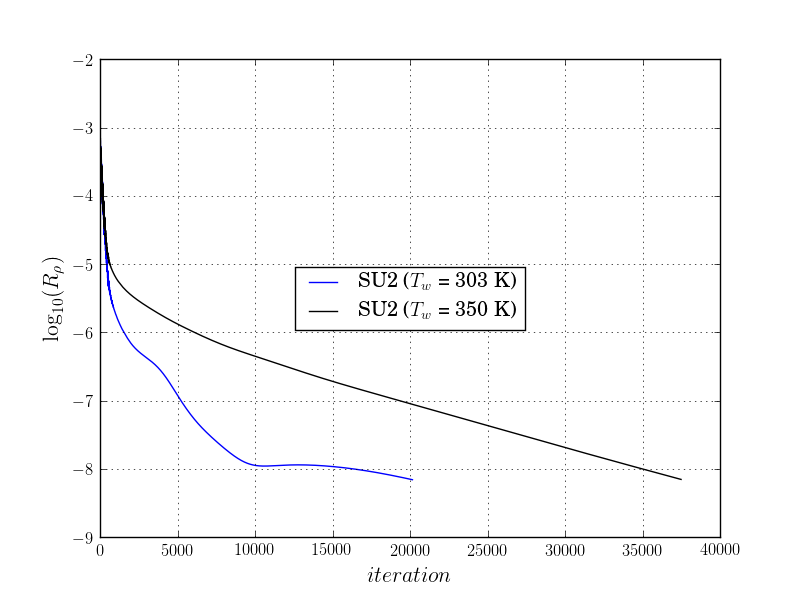
\includegraphics[width=\linewidth]{residuals.png}
\caption{The convergence history of the density residual, $R_\rho$, for both simulations.}
\label{fig:rho_res}
\end{figure}

\subsection*{Skin Friction}
Fig.~\ref{fig:cf} compares the coefficients of skin friction, $C_f$, calculated by SU2 with that of the analytical solution by Blasius:

\begin{equation*}
C_f(x) = \dfrac{0.6641}{\sqrt{Re_x}},
\end{equation*}

where $Re_x = \tfrac{U_\infty x}{\nu}$ is the local Reynolds number. Checking the skin friction coefficient is generally a good way of assessing the quality of a laminar, flat-plate simulation.

\begin{figure}[h] 
\centering
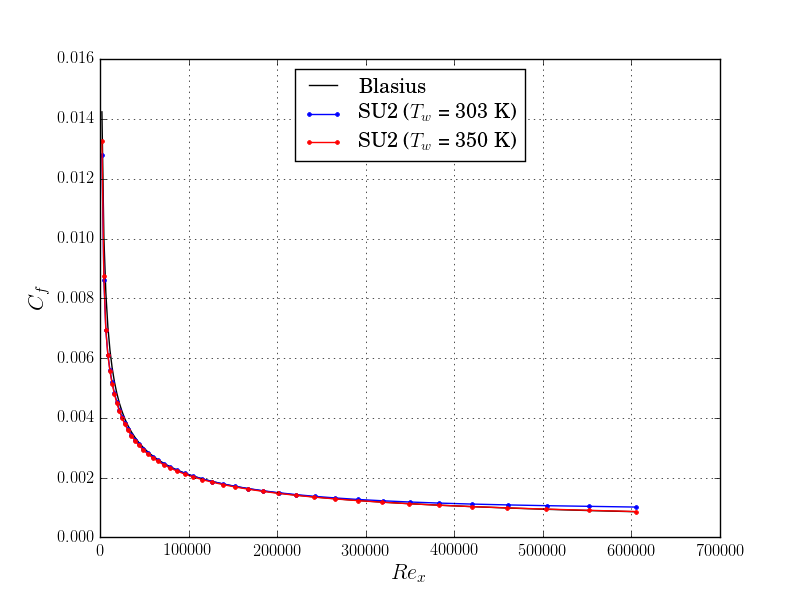
\includegraphics[width=\linewidth]{cf.png}
\caption{Variation in $C_f$ along the length of the plate plotted as a function of local $Re$.}
\label{fig:cf}
\end{figure}

\subsection*{Thermal Boundary Layer}
The isothermal wall condition allows one to investigate the development and growth of a thermal boundary layer along the surface of the plate. In Fig.~\ref{fig:temp}, nondimensionalized temperature, 

\begin{equation*}
\theta = \dfrac{T-T_w}{T_\infty-T_w},
\end{equation*}

has been plotted against nondimensionalized wall distance,

\begin{equation*}
\eta = \dfrac{y}{\sqrt{\dfrac{\nu x}{U_\infty}}},
\end{equation*}

where $\nu = \mu/\rho$ denotes the kinematic viscosity. In Fig.~\ref{fig:temp}, the cross-section has been taken along the outlet boundary --- i.e. at the end of the plate.

The temperature profiles extracted from the SU2 output are compared against the analytical solution of Pohlhausen as well as the Crocco-Busemann relation, which is designed to account for the effects of compressibility. Pohlhausen's solution is given by

\begin{equation*}
\theta_{Pohlhasusen} = 1 - \dfrac{\mathlarger{\int_{\eta}^{\infty}}\mathsmaller{\left( \dfrac{d^2f}{d\eta^2}\right)}^{Pr}d\eta}{\mathlarger{\int_{0}^{\infty}}\mathsmaller{\left( \dfrac{d^2f}{d\eta^2}\right)}^{Pr}d\eta},
\end{equation*}

where $f$ is the well-known solution to the Blasius equation. The Crocco-Busemann relation is given in terms of temperature at a given point in the domain, namely:

\begin{equation*}
T_{CB} = T_w + \left( T_{aw}-T_w \right)\frac{u}{U_\infty} - \dfrac{ru^2}{2c_p}.
\end{equation*}

Here, $u$ is the local velocity in the $x$ direction, $r$ is the so-called ``recovery factor" given by $r = \sqrt{Pr}$, and $T_{aw}$ denotes the \textit{adiabatic wall temperature}, defined as

\begin{equation*}
T_{aw} = T_\infty + \dfrac{rU_\infty^2}{2c_p}.
\end{equation*}

In Fig.~\ref{fig:temp}, the temperature given by the Crocco-Busemann model, $T_{CB}$, has been nondimensionalized as follows:

\begin{equation*}
\theta_{CB} = \dfrac{T_{CB}-T_w}{T_\infty-T_w}.
\end{equation*}

\begin{figure}[h] 
\centering
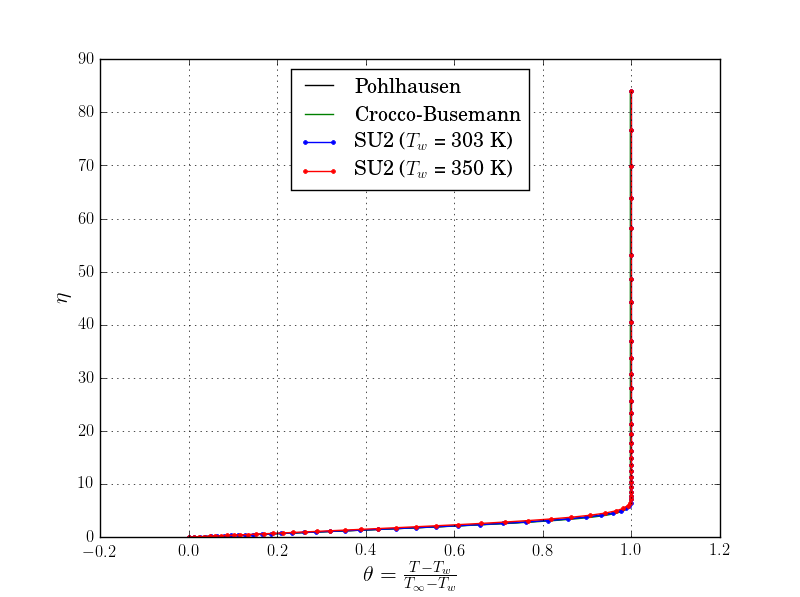
\includegraphics[width=\linewidth]{temp.png}
\caption{Nondimensionalized temperature profiles at the outlet.}
\label{fig:temp}
\end{figure}

Fig.~\ref{fig:temp_zoom} redraws the temperature profiles seen in Fig.~\ref{fig:temp} but shows the boundary-layer region in much more detail.
 
\begin{figure}[h] 
\centering
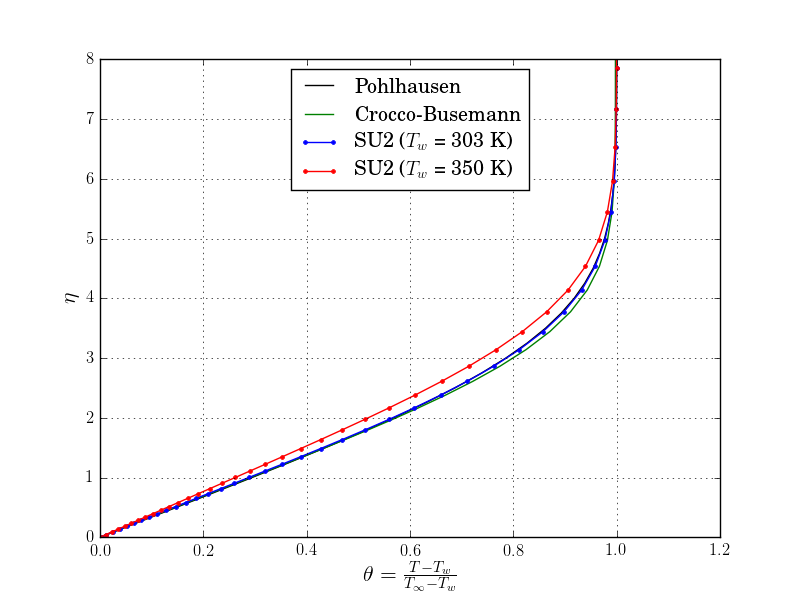
\includegraphics[width=\linewidth]{temp_zoom.png}
\caption{Profiles in Fig.~\ref{fig:temp} magnified near the boundary layer. N.B. The solution of Pohlhausen falls directly atop the computational result for $T_w = \SI{303}{\kelvin}$.}
\label{fig:temp_zoom}
\end{figure}

\subsection*{Nusselt Number}
The rate of heat transfer along the surface of the plate, $q_w$, was calculated by SU2 and used to compute a distribution of local Nusselt number,

\begin{equation*}
Nu_x = -\dfrac{q_wx}{k\left(T_w-T_\infty\right)}.
\end{equation*} 

Fig.~\ref{fig:Nu} compares the results from simulation with the analytical solution of Blasius, viz.

\begin{equation*}
Nu_{x_{Blasius}} = 0.332\sqrt{Re_x}Pr^{1/3}.
\end{equation*} 

\begin{figure}[h] 
\centering
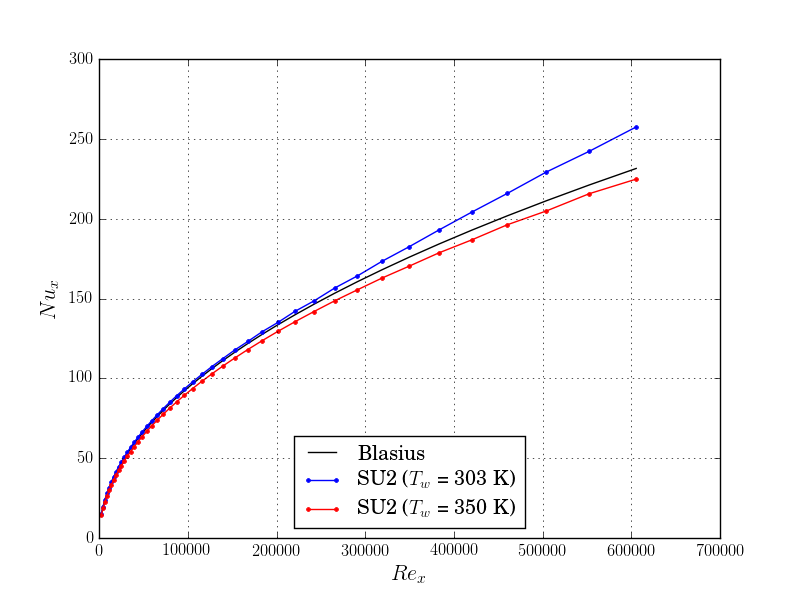
\includegraphics[width=\linewidth]{nu.png}
\caption{Local Nusselt number plotted along the length of the plate.}
\label{fig:Nu}
\end{figure}

\subsection*{Density Variation}
Naturally, when using a compressible solver, changes in temperature will lead to changes in density. Lest comparisons to the incompressible Blasius solutions be suspect, Fig.~\ref{fig:rho} shows how the flow density varies through the boundary layer at the trailing edge of the plate. Whether or not this change in density is too large for a comparison to be made between these simulations and the Blasius solutions is a matter of the analyst's discretion.

\begin{figure}[h] 
\centering
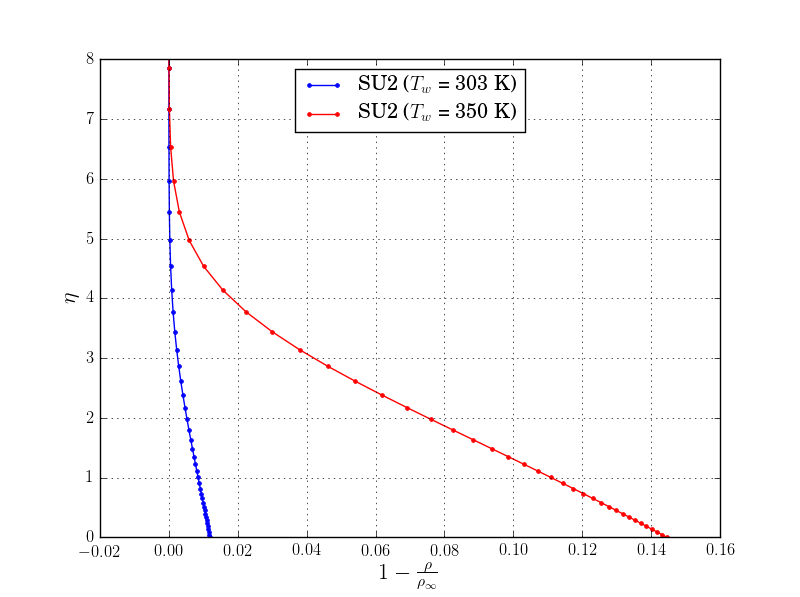
\includegraphics[width=\linewidth]{rho.png}
\caption{Density profiles observed at the mesh outlet.}
\label{fig:rho}
\end{figure}

\section*{Summary}
Some of the salient results from two isothemeral, laminar, flat-plate simulations have been presented. When deemed appropriate, CFD results from SU2 have been compared against the analytical solutions of Blasius, Pohlhausen, and Crocco-Busemann. On balance, it appears that prescribing a small temperature difference, $T_w-T_\infty$, as well as a low inlet Mach number allows the output from a compressible solver to be reasonably compared with incompressible analytical results. This appears to be the case for both aerodynamics as well as heat transfer.

\end{document}